\section{Introduction}
\label{sec:introduction}

The phenomenon of online ticket sales for large-scale events has become a major highlight in the digital industry. Events like the Taylor Swift's "The Eras Tour" demonstrate the immense technical challenges, where platforms like Ticketmaster faced failures due to demand surges, with millions of users vying for a limited number of tickets simultaneously \cite{swiftTicketmaster}. This highlights a fundamental technical challenge: designing a system capable of handling millions of concurrent users without failure.

The scalability of ticketing systems has unique characteristics. Users arrive exponentially in a short period, demanding the system to handle spikes in both read operations (checking ticket availability) and write operations (processing orders). Furthermore, resource contention is extreme as many users attempt to book the same seats. While various architectural approaches like event-driven architecture, database sharding, and flow control mechanisms exist, there is limited specific research on the combined performance of these approaches in extreme-demand scenarios for ticketing systems.

This research aims to fill this gap by investigating and testing various architectural approaches to formulate an optimal and reliable solution for ticket sales systems. The main contribution of this paper is a comprehensive performance comparison of different distributed relational database architectures and the evaluation of flow control strategies in maintaining system stability and performance under high-load conditions. The objective is to analyze the throughput, latency, and resource usage of a standard PostgreSQL cluster, CitusData, and YugabyteDB, and to evaluate the effectiveness of flow control in stabilizing order processing. This study is limited to open-source solutions and focuses on a single-event, single-region sales scenario, without go through into user experience aspects like virtual queues or failover testing.

\section{Methods and Materials}
\label{sec:methods}
This study evaluates different architectural solutions for a high-traffic ticketing system. The system is modeled ticket and payment services, focusing on backend performance rather than user interface.

\subsection{Literature Review}
The core of high-load systems often lies in database scalability. Traditional relational databases scale vertically, which has physical and cost limitations. This research explores horizontally scalable relational databases.
\begin{itemize}
    \item \textbf{Database Scaling Techniques}: We reviewed leader-follower replication, which enhances read throughput but leaves the leader as a write bottleneck, and partitioning (sharding), which distributes data and load across nodes \cite{dataIntensiveApplications}.
    \item \textbf{Distributed Relational Databases}: We selected three PostgreSQL-compatible databases to represent different architectures:
          \begin{enumerate}
              \item \textbf{PostgreSQL Cluster}: A standard primary-replica setup serves as the baseline.
              \item \textbf{CitusData}: An extension that transforms PostgreSQL into a distributed database with a coordinator-worker architecture, enabling parallel query processing and multiple-writer \cite{citus}.
              \item \textbf{YugabyteDB}: A distributed SQL database built from the ground up, using the Raft consensus protocol for high availability and native distribution, compatible with the PostgreSQL API \cite{yugabyte}.
          \end{enumerate}
    \item \textbf{Flow Control}: To manage backpressure from high request volumes, we investigated the Queue-Based Load Leveling pattern. This pattern uses a queue as a buffer to decouple tasks from services, allowing the system to process messages at a consistent rate, thus ensuring stability \cite{queueLoadLeveling}.
    \item \textbf{Supporting Technologies}: \textbf{Redis} was chosen for its high-speed, in-memory key-value store capabilities, ideal for caching frequently accessed data like ticket availability aggregates. \textbf{RabbitMQ} was selected as the message broker for its reliability and support for the queueing pattern needed in the flow control mechanism.
\end{itemize}

\subsection{System Design and Methodology}
The problem was broken down into four key challenges: transaction processing rate, read query processing, data integrity, and system stability.

\begin{enumerate}
    \item \textbf{Increasing Transaction Throughput}: To overcome the write limitations of a single primary database, we designed and compared three database architectures: a baseline PostgreSQL cluster, a CitusData cluster, and a YugabyteDB cluster. The goal was to evaluate their ability to scale out write operations.

    \item \textbf{Optimizing Read Operations}: For high-volume read queries like checking seat availability, a multi-layered caching strategy was designed. Aggregated availability data (e.g., number of seats left in a section) was cached in a Redis cluster for fast, low-latency access. For granular seat-level availability, a short-lived in-memory cache at the application level was used to reduce direct database hits.

    \item \textbf{Ensuring Data Integrity}: To prevent double-booking, the system leverages the transactional capabilities of relational databases. Row-level locking (`SELECT ... FOR UPDATE`) is used within transactions to ensure that a seat being booked by one user cannot be accessed by another concurrent transaction until the first one is completed.

    \item \textbf{Implementing Flow Control}: A flow control scheme was designed to maintain stability. This involved two strategies:
          \begin{itemize}
              \item \textbf{Early Request Rejection}: A pre-check against Redis is performed to reject booking requests for seats that are already sold or are currently being processed in the queue, reducing unnecessary load on the database.
              \item \textbf{Queued Order Processing}: Booking requests are placed into a RabbitMQ queue. A separate pool of workers processes these requests at a controlled rate, preventing the database from being overwhelmed by request spikes.
          \end{itemize}

\end{enumerate}

\subsection{Testing Plan}
A rigorous testing methodology was designed to simulate real-world, high-demand scenarios.
\begin{itemize}
    \item \textbf{Load Simulation}: The K6 load testing tool was used to generate traffic from thousands of virtual users (VUs).
    \item \textbf{User Behavior}: VUs were assigned diverse profiles, varying in ticket category preference, purchase quantity, and persistence in retrying failed attempts, to mimic realistic buyer behavior.
    \item \textbf{Test Scenarios}: Two primary scenarios were executed:
          \begin{enumerate}
              \item \textbf{Sustained Load Test}: The system was subjected to a constant high number of VUs (10,000-15,000) for a sustained period (10-15 minutes) to test its stability and throughput under continuous stress.
              \item \textbf{Ticket Scramble (Spike Test)}: This scenario simulated a "ticket drop" with a log-normal arrival rate of users, creating a massive initial spike in traffic to test the system's ability to handle sudden, extreme demand.
          \end{enumerate}
    \item \textbf{Monitoring}: The system was monitored using a stack of Prometheus for metrics collection and Grafana for visualization, tracking CPU/memory usage, latency, error rates, and database query performance.
\end{itemize}

\section{Results and Discussion}
\label{sec:results}

\subsection{Performance of Distributed Databases}
The performance of the three database architectures varied significantly under high load. A summary of the performance during the sustained load test is presented in Table \ref{tab:perf_summary}.

\begin{table}[H]
    \caption{Overall Performance of Order Processing}
    \label{tab:perf_summary}
    \centering
    \begin{tabular}{|l|c|c|c|}
        \hline
        \textbf{Metric} & \textbf{PostgreSQL} & \textbf{CitusData} & \textbf{YugabyteDB} \\
        \hline
        Max Throughput  & 466 rps             & 410 rps            & 216 rps             \\
        \hline
        Peak CPU Usage  & 8 vCPU              & 10 vCPU            & 19 vCPU             \\
        \hline
        Peak Memory     & 3.4 GB              & 5 GB               & 36 GB               \\
        \hline
        Latency (P50)   & 192-382 ms          & 496-650 ms         & 854-10000 ms        \\
        \hline
    \end{tabular}
\end{table}

\begin{itemize}
    \item \textbf{PostgreSQL Cluster}: The baseline PostgreSQL cluster demonstrated excellent performance. It handled the load with the lowest latency, highest throughput, and most efficient resource utilization. Its monolithic architecture avoided the network and coordination overhead inherent in distributed systems, proving highly effective for the workload characterized by numerous small, fast transactions.

    \item \textbf{CitusData}: CitusData showed acceptable performance, with throughput approaching that of PostgreSQL but with significantly higher latency (approx. 2x) and greater resource consumption. The overhead was largely attributed to the coordinator node, which became a bottleneck for query planning and coordination, especially since the workload consisted of many simple queries rather than complex analytical ones \cite{Slot2020}.

    \item \textbf{YugabyteDB}: YugabyteDB performed poorly. It had less than half the throughput of PostgreSQL, latency that was at least 4x higher, and vastly greater CPU (2.4x) and memory (10x) usage. The cluster exhibited instability under higher loads, with high failure rates and inconsistent performance. The inherent latency of its Raft-based consensus mechanism proved detrimental for this type of high-contention, low-latency transactional workload.

\end{itemize}

\subsection{Effectiveness of Read Query Optimization}
The read optimization strategies yielded mixed results.
\begin{itemize}
    \item The use of \textbf{Redis for caching aggregated area availability} was highly effective. This endpoint handled up to 1700 rps with an average latency of just 2.5-4.5 ms, successfully offloading significant read traffic from the primary database.
          \begin{figure}[H]
              \centering
              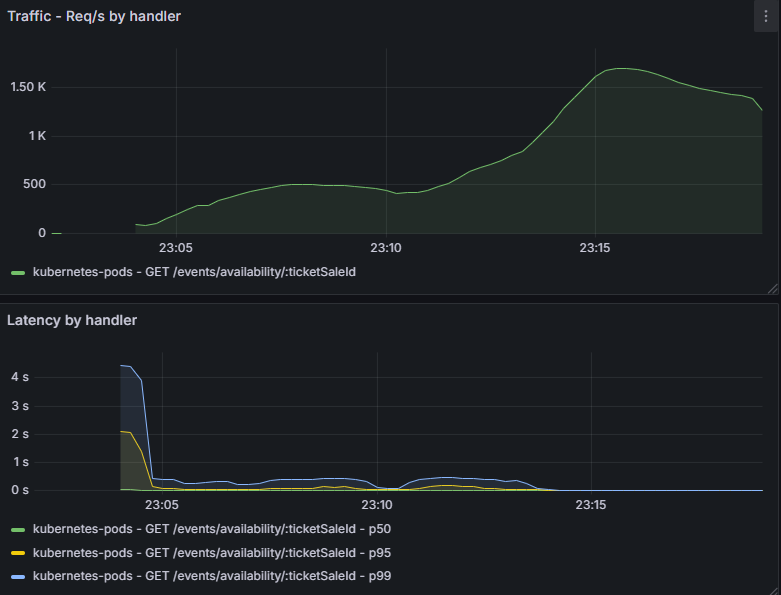
\includegraphics[width=0.35\textwidth]{resources/chapter-4/latency-area-availability.png}
              \caption{Read Area Availability Metrics}
              \label{fig:latency-get-area}
          \end{figure}

    \item The \textbf{in-memory micro-caching for individual seat availability} was not effective. The cache hit ratio was very low due to the local nature of the cache (per application instance), the wide distribution of requests across different areas, and the short cache lifetime (150 ms). This resulted in high P95 latencies (up to 7 seconds), indicating that this remains a bottleneck.
          \begin{figure}[H]
              \centering
              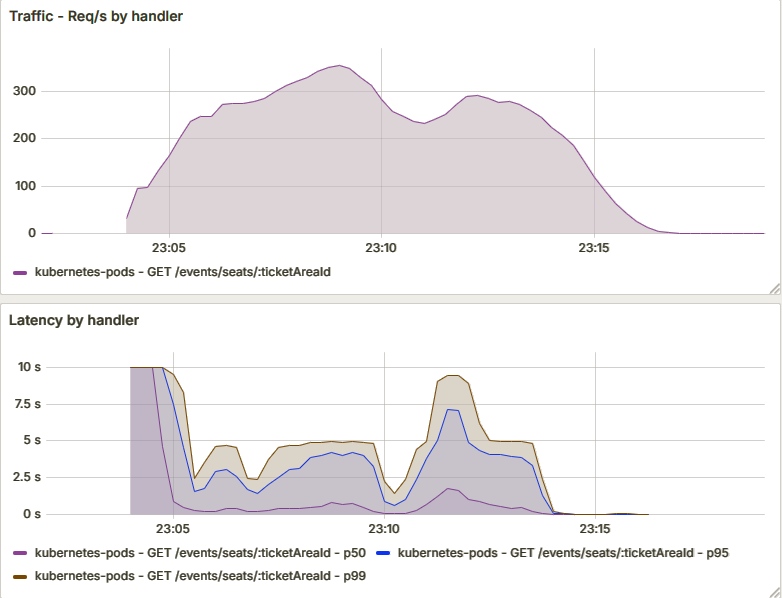
\includegraphics[width=0.35\textwidth]{resources/chapter-4/latency-seat-availability.png}
              \caption{Read Seat Availability Metrics}
              \label{fig:latency-get-seat}
          \end{figure}
\end{itemize}

\subsection{Impact of Flow Control}
The flow control mechanism demonstrated significant benefits, particularly in reducing database load.
\begin{itemize}
    \item \textbf{Early request rejection} using Redis was highly effective. It successfully filtered out requests for unavailable seats before they hit the database, reducing the latency for failed booking attempts from 1-2 seconds down to 50-100 milliseconds.
          \begin{figure}[H]
              \centering
              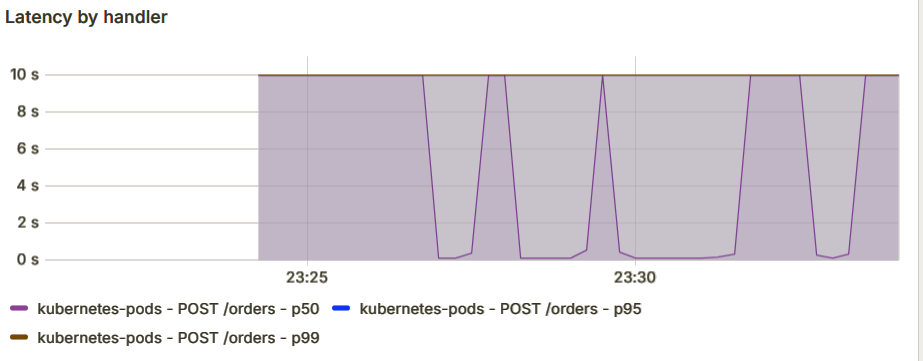
\includegraphics[width=0.45\textwidth]{resources/chapter-4/latency-fc-pg-stress-0.png}
              \caption{Processing Latency with Flow Control}
              \label{fig:latency-fc}
          \end{figure}

          \begin{figure}[H]
              \centering
              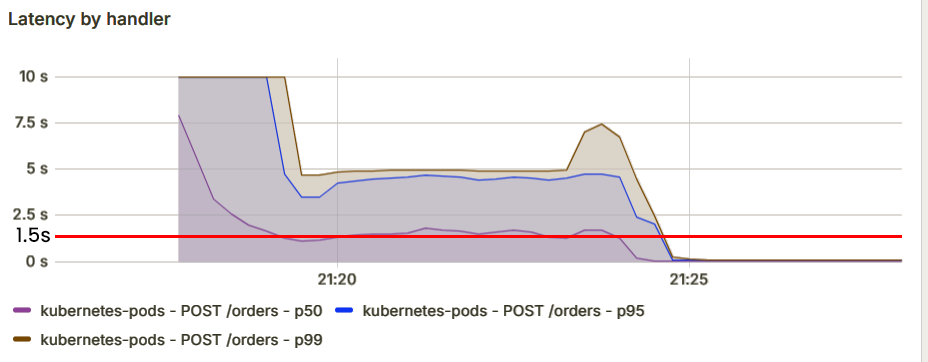
\includegraphics[width=0.45\textwidth]{resources/chapter-4/latency-nofc-pg-stress-0.png}
              \caption{Processing Latency without Flow Control}
              \label{fig:latency-nofc}
          \end{figure}
    \item The \textbf{queue-based processing} showed potential but was hampered by the high latency introduced by RabbitMQ. While it successfully smoothed out the load on the database and reduced contention (evidenced by lower query latency for locking), the overall end-to-end latency for the user was much higher. The test load was also not high enough to create a scenario where the baseline PostgreSQL system was completely overwhelmed, which is where this pattern would provide the most benefit.
          \begin{figure}[H]
              \centering
              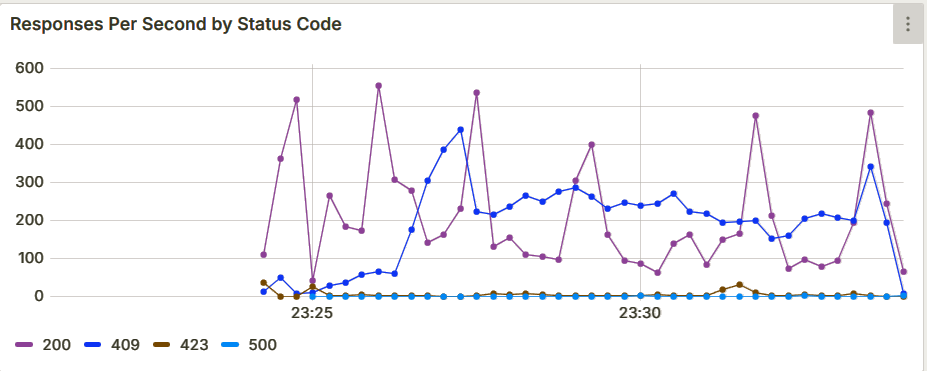
\includegraphics[width=0.45\textwidth]{resources/chapter-4/rps-fc-pg-stress-0.png}
              \caption{Transaction Processing Rate with Flow Control}
              \label{fig:rps-fc-pg-stress-0}
          \end{figure}

          \begin{figure}[H]
              \centering
              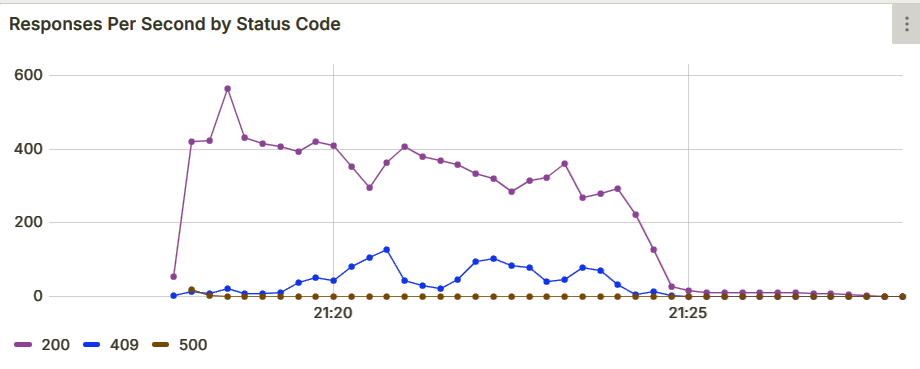
\includegraphics[width=0.45\textwidth]{resources/chapter-4/rps-nofc-pg-stress-0.png}
              \caption{Transaction Processing Rate without Flow Control}
              \label{fig:rps-nofc-pg-stress-0}
          \end{figure}
\end{itemize}

\pagebreak

\subsection{Data Integrity}
Throughout all tests, including the high-contention ticket scramble scenario, the system maintained perfect data integrity. Sanity checks confirmed that there were no instances of double-booked seats, and the data between Redis and the database remained eventually consistent. This validates the robustness of using transactional row-level locking in the relational database to handle race conditions.

\section{Conclusion and Future Work}
\label{sec:conclusion}
This research concludes that for high-contention, transactional workloads like large-scale ticket sales, a well-tuned monolithic relational database like \textbf{PostgreSQL with read replicas offers superior performance and resource efficiency} compared to the tested distributed SQL solutions. The overhead of coordination and consensus in CitusData and YugabyteDB outweighs their horizontal scaling benefits for this specific use case.

Optimizing read operations by offloading aggregate queries to an in-memory store like Redis is a highly effective strategy. However, fine-grained caching requires a more sophisticated approach than simple, short-lived local caches. Flow control, particularly early request rejection, is crucial for reducing unnecessary database load and improving system stability. While queue-based processing can protect the database, its implementation must carefully manage the trade-off with end-to-end latency.

Future work should focus on:
\begin{enumerate}
    \item Exploring more advanced caching strategies for granular data.
    \item Implementing a lower-latency queueing mechanism, possibly at the application level, to reduce the overhead seen with RabbitMQ.
    \item Testing the architectures under even higher loads (e.g., \textgreater
          100,000 VUs) to find the breaking point of the monolithic PostgreSQL setup and determine where a distributed solution like CitusData, perhaps with optimizations like stored procedures, becomes necessary.
    \item Separating connection pools for read and write operations to further reduce contention on the primary database instance.
\end{enumerate}

\section{Availability}
The complete thesis, including the source code for the system implementation and load testing scripts, is publicly available in the author's GitHub repository: \url{https://github.com/akbarmridho/tugas-akhir}.